
%----------------------------------------------------------------------------------------
%	PACKAGES
%----------------------------------------------------------------------------------------
\documentclass{article}
\usepackage[utf8]{inputenc}
\usepackage[version=3]{mhchem} % Package for chemical equation typesetting
\usepackage{siunitx} % Provides the \SI{}{} and \si{} command for typesetting SI units
\usepackage{graphicx} % Required for the inclusion of images
\usepackage{natbib} % Required to change bibliography style to APA
\usepackage{amsmath} % Required for some math elements 
\usepackage{wrapfig}
\usepackage[top=2cm,left=2cm,bottom=2cm,right=2cm]{geometry}
\usepackage[table]{xcolor}
\usepackage{float}
%----------------------------------------------------------------------------------------
%	INFORMATION DU DOCUMENT
%----------------------------------------------------------------------------------------

\title{Compte rendu de travaux pratiques de l'UE \\Apprentissage et Reconnaissances des Formes} % Title
\author{Asma \textsc{BRAZI} 3703554 \\ Wang \textsc{Tingbo} 3770815} % Author name
\date{Année universitaire 2018/2019}

%----------------------------------------------------------------------------------------
%	CONTENU DU DOCUMENT
%----------------------------------------------------------------------------------------
\begin{document}
\maketitle
\begin{center}
\rule{0.7\textwidth}{.4pt}
\end{center}
%----------------------------------------------------------------------------------------
%	INTRODUCTION
%----------------------------------------------------------------------------------------
\begin{abstract}
Ce rapport a pour objectif de présenter le travail que nous avons effectué, dans le cadre des travaux pratiques de l'UE ARF (Apprentissage et Reconnaissance des formes). Nous y rassemblons nos expériences, nos résultats et nos observations.\\
Chaque section concerne ....
\end{abstract}


\section{Objectif}
\quad Notre objectif et d'étudier des méthodes quantitatives en Intelligence Artificielle et en reconnaissance des formes. Pour commencer, nous abordons les arbres de décision. Ensuite, 

\section{Analyse}
%----------------------------------------------------------------------------------------
%	ARBRES DE DÉCISION
%----------------------------------------------------------------------------------------

\subsection{Arbres de décision}


\begin{wrapfigure}{r}{0.2\textwidth}
  \vspace{-20pt}
  \begin{center}
    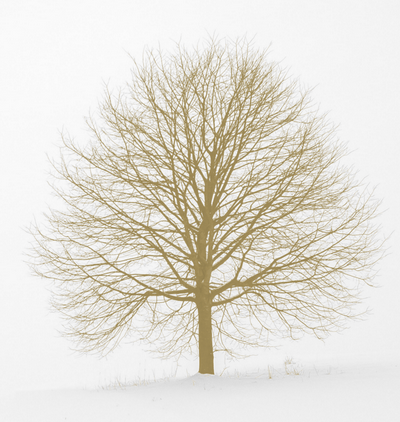
\includegraphics[width=0.2\textwidth]{tree.png}
  \end{center}
  \vspace{-20pt}
  \vspace{-10pt}
\end{wrapfigure}
\quad Un arbre de décision est un modèle de classification hiérarchique. Il est est constitué de noeuds, d'arcs et de feuilles. Au niveau de chaque noeud, un attribut est testé. Puis, les arcs correspondent au résultat d'un test puis mènent vers le prochain attribut à tester, ou bien à une feuille.La feuille est un noeud terminal prédit le résultat. \\Afin de sélectionner le meilleur attribut à chaque niveau,\\ nous calculons l'entropie de Shannon qui pour caractériser le degré de désorganisation ou d'imprédictibilité d’un échantillon. \\
Pour résumer, lorsque nous avons un nouvel exemple qui se présente, il sera classé, en le soumettant à une séquence de tests. À la fin de ces tests,la classe à laquelle appartient l'exemple est déterminée. 

\subsubsection{Expérience préliminaires sur le modèle}
\quad Pour commencer, nous allons étudier dans cette partie l'impact de la profondeur de l'arbre sur le nombre  d'exemples générés au niveau des feuilles. Pour cela nous allons varier la valeur de la profondeur de l'arbre et voir son impact.
\linebreak
\linebreak
\begin {center}
\begin{tabular}{|c|c|c|c|c|}
  \hline \rowcolor{lightgray}
  Profondeur & 3 & 5 & 10 & 20 \\
  \hline
  Score & 0.71 & 0.73 & 0.82 & 0.89 \\
  \hline
\end{tabular}
\end {center}


Tout d'abord, le nombre d'exemples générés croit (resp décroît) lorsque la profondeur de l'arbre augmente (resp diminue). Puis, le score obtenu augmente aussi lorsque nous augmentons la profondeur de l'arbre. Car cette dernière spécialise la classification. En revanche, un score trop élevé limite les capacités de généralisation.
\linebreak
\linebreak
 Nous précisions que ces scores ne sont guère un indicateur fiable du comportement de l’algorithme, puisque ces évaluations ont été réalisées sur les données d’apprentissage. Afin d'obtenir un indicateur fiable, nous divisons notre base en deux sous-ensembles. Le premier sous-ensemble correspondrait à l'ensemble d'apprentissage et le second à l'ensemble de test.
 
%----------------------------------------------------------------------------------------
%	SUR SOUS-APPRENTISSAGE
%----------------------------------------------------------------------------------------


\subsubsection{Sur et sous apprentissage}
Dans cette partie, nous allons effectuer différents partitionnement de l'ensemble initial en un ensemble d'apprentissage et un ensemble de test. À savoir: (0.2, 0.8), (0.5, 0.5) et (0.8, 0.2). Nous traçons les courbes de l'erreur en apprentissage et de l’erreur en test en fonction de la profondeur du
modèle. 

\begin{figure}[H]
  \begin{center}
    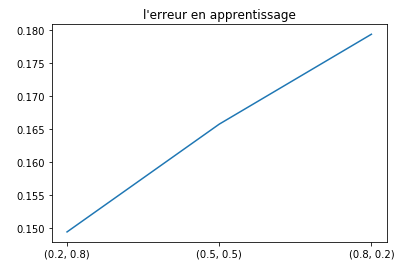
\includegraphics[width=0.6\textwidth]{erreur_app_part.png}
    \caption{Courbe de l’erreur en apprentissage pour différentes partitionnements de l'ensemble des données}
  \end{center}
\end{figure}


\begin{figure}[H]
  \begin{center}
    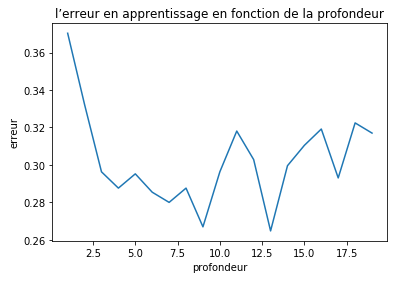
\includegraphics[width=0.6\textwidth]{erreur_app.png}
    \caption{Courbe de l’erreur en apprentissage en fonction de la profondeur de l'arbre}
  \end{center}
\end{figure}

\begin{figure}[H]
	\begin{center}
		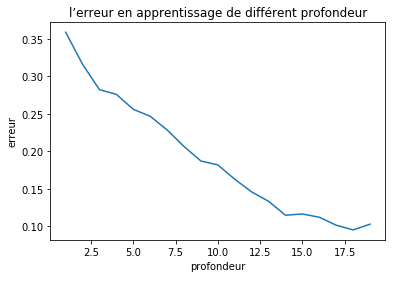
\includegraphics[width=0.6\textwidth]{erreur_test.png}
		\caption{Courbe de l’erreur en test en fonction de la profondeur de l'arbre}
	\end{center}
\end{figure}


Quand il y a peu d'exemples d'apprentissage, le score de prédiction est faible car le modèle n'apprend pas suffisamment. D'ailleurs, nous sommes presque dans l'aléatoire. Dans le cas contraire, lorsqu'il y a beaucoup d'exemples d'apprentissage, le modèle sur-apprend et il sera pas très bon à la prédiction car il ne sera pas très bon à la généralisation. Par conséquent, nous obtenons un score faible à la prédiction. D'où une faible performance.

\begin{figure}[H]
  \begin{center}
    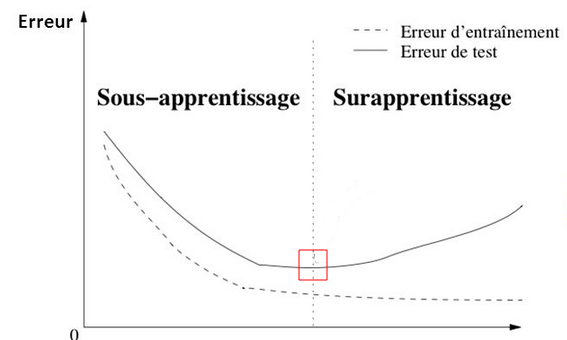
\includegraphics[width=0.8\textwidth]{apprentissage.png}
    \caption{Mémorisation de l'ensemble d'apprentissage}
  \end{center}
\end{figure}
Il est inévitable de trouver un compromis entre le sur-apprentissage et le sous-apprentissage, où le modèle est bon sur ces deux ensembles. Sur la figure ci-dessus, le point que nous cherchons à atteindre est encadrer 

Comme solution, nous pourrons considérer un ensemble de validation. Ceci reste une méthode simple et efficace. Ce qui permet d'entraîner et de tester le modèle K fois sur différents sous-ensembles et d'estimer la performance sur de nouvelles données.


%----------------------------------------------------------------------------------------
%	VALIDATION CROISÉE
%----------------------------------------------------------------------------------------
\subsubsection{Validation croisée}


\quad Comme nous espérons obtenir des résultats plus fiables et stables, nous cherchons à utiliser la base initiale de données complètement. Pour cela, la méthode de la validation croisée nous permet de tester à quel point notre modèle est efficace sur un ensemble de validation supposé. Surtout, lorsque nous avons pas un ensemble de validation explicite. La méthode consiste à partitionner notre base de données en N partitions. Puis, nous effectuons N itérations où à chaque tour de boucle, nous considérons la ième partition comme une base de test et les autres partitions restantes comme une base d'apprentissage.

\begin{figure}[H]
  \begin{center}
    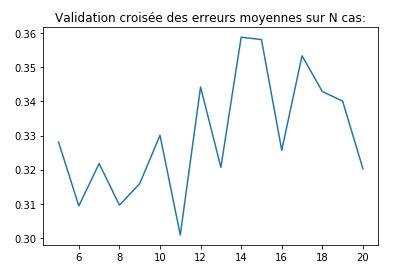
\includegraphics[width=0.6\textwidth]{cross_courbe.png}
    \caption{Courbe des erreurs moyennes sur N cas}
  \end{center}
\end{figure}

L'expérience dont les résultats se résument dans la figure ci-dessus nous montre que lorsque la profondeur est égale à 11, nous obtenons les meilleurs résultats.

%----------------------------------------------------------------------------------------
%	ESTIMATION DE DENSITÉ
%----------------------------------------------------------------------------------------

\subsection{Estimation de densité}
La densité de probabilité décrit la distribution des données dans l'espace vectoriel. Ceci nous permet une meilleure maîtrise des caractéristiques de ces données, à travers les régions les couvrant.\\\\
L'étude que nous menons, consiste à estimer la loi de densité géographique des points d'intérêts sur Paris. Plus précisément pour le POI textbf{atm}. \\\\
\\Dans le cadre du module, nous étudions deux méthodes d'estimation de densité: la méthode des histogrammes et la méthode à noyaux.

\subsubsection{Méthode des histogrammes}
Cette méthode représente la répartition des données à l'aide des histogrammes, pour approximer la fonction de densité.
Dans notre étude, nous discrétisons la carte géographique en comptant le nombre d'observations appartement à chaque région. 


\subsubsection{Méthode à noyaux}
\paragraph{}
La méthode à noyaux consiste à retrouver la continuité que nous perdons dans la méthode des histogrammes. En effet, grace au paramètre \textbf{h} que nous fixons, l'estimation peut devenir lisse. Cependant, un exemple proche du point de support \textbf{x} se voit attribué une grande valeur et vis-versa. 
\subsubsection{Éxpériences}
\paragraph{}
Nous allons effectuer quelques expériences sur l'estimation de densité par différentes méthodes. Pour commencer, nous allons étudier la méthode des histogrammes en variant la largeur de chaque bin de l'histogramme.

\begin{figure}[H]
	\begin{center}
		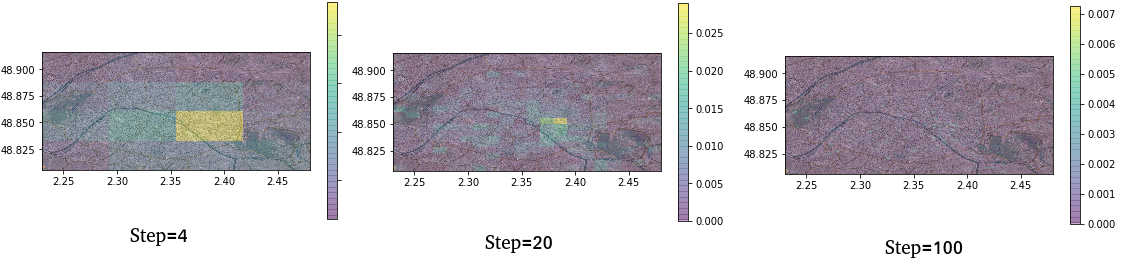
\includegraphics[width=0.8\textwidth]{histo.png}
		\caption{Estimation de densité par la méthode des histogrammes }
	\end{center}
\end{figure}
\paragraph{}
Nous remarquons que lorsque nous fixons le pas de discrétisation à une grande valeur, la précision devient pointilleuse créant des discontinuités. Cependant, ceci rend le modèle incapable de généraliser.Nous dirons que le modèle sur-apprend.
\paragraph{}
Dans le cas contraire, un faible pas de discrétisation regroupe les données dans de larges bins. Ceci résulte une faible précision. Aussi, Comme ces données ne partagent pas forcément les mêmes caractéristiques, alors  nous nous retrouvons dans un abus de généralisation. Le modèle sous-apprend.
\paragraph{}
Maintenant, nous allons étudier la méthode à noyaux. Les noyaux implémentés sont Parzen et et Gauss.
\begin{figure}[H]
	\begin{center}
		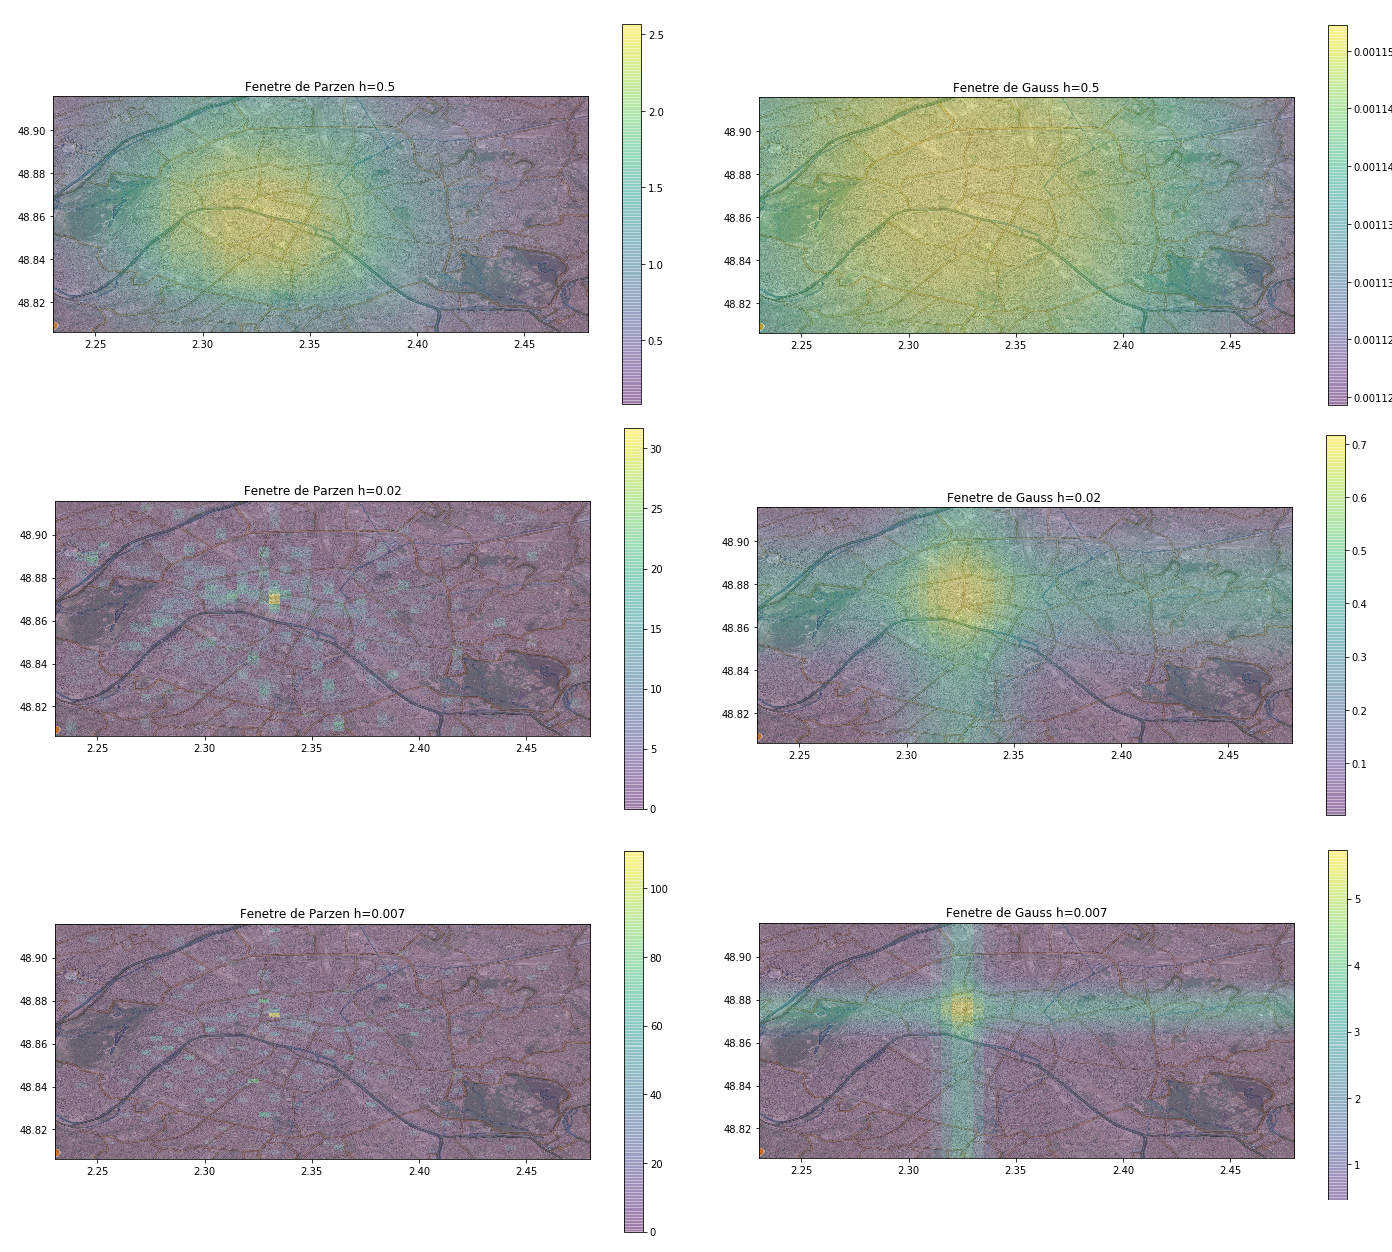
\includegraphics[width=1\textwidth]{parzen_vs_gauss.png}
		\caption{Estimation de densité par la méthode à noyaux (Parzen et Gauss)}
	\end{center}
\end{figure}
\paragraph{}
À la différence de la méthode des histogrammes, la méthode à noyaux considère le voisinage du point courant que l'on souhaite lui approcher sa densité pour éviter la discrétisation. Ce voisinage est déterminé par les paramètres du modèle.
\paragraph{}
Après avoir étudié plusieurs cas de figure en variant le paramètre \textbf{h}. Nous concluons qu'avec une base d'observations importante, il serait nécessaire de fixer un \textbf{h} grand pour un lissage important. 
\end{document}